\documentclass{article}
\usepackage[utf8]{inputenc}
\usepackage{amsmath, amsthm}
\usepackage{parskip}
\usepackage{graphicx}

\usepackage{XCharter}
\usepackage[charter]{mathdesign}

\usepackage{amsmath}

\DeclareMathOperator{\range}{range}
\DeclareMathOperator{\nul}{null}
\DeclareMathOperator{\im}{im}


\begin{document}
\title{MG tutorial notes}
\author{Gabriel Clave}
\maketitle

\tableofcontents

\section{Relaxation methods}

\subsection{Notations}

\begin{align*}
    \text{Problem:}          \quad & Au = f \\
    \text{Error:}            \quad & e = u - v \\
    \text{Residual:}         \quad & r = f - Av \\
    \text{Residual Problem:} \quad & Ae = r
\end{align*}

\subsection{Matrix splitting}

Decompose $A$ into $M - N$, where $M$ is easy to invert.

\[
    Au = f \implies Mu = Nu + f
\]

$u$ is a stationary point:
\[
    u = M^{-1}Nu + M^{-1}f
\]

With $S = M^{-1}N = I - M^{-1}A$, we use the iteration:
\[
    v^{(k+1)} = Sv^{(k)} + M^{-1}f
\]

Using $M^{-1}f = u - Su$, we get:
\[
    e^{(k+1)} = Se^{(k)} = S^{k}e^{(0)}
\]

If $\|S\| < 1$, the error is forced to zero.

the iterate can also be expressed as:
\[
    v^{(k+1)} = v^{(k)} + M^{-1}r
\]

% look for more general case with preconditioner

\subsubsection*{Examples (for matrices with nonzero diagonal)}
\begin{itemize}
    \item \textbf{Jacobi:} $A = D - L - U \quad M = D$
    
    \[
        Dv^{(k+1)} = (L + U)v^{(k)} + f
    \]
    \[
        a_{ii}v^{(k+1)}_{i} = \sum_{j \neq i}a_{ij}v^{(k)}_{j} + f_{i}
    \]
    solve for $v_{i}$ using the previous estimate

    \item \textbf{Gauss-Seidel:} $M = D - L$
    \[
        (D-L)v^{(k+1)} = Uv^{(k)} + f
    \]
    
    solve for $v_{j}$ using the previous estimate and already computed values
\end{itemize}

\subsubsection*{Issue \& strength}
Very slow convergence rate: good at the beginning, then stagnates. \\ 
Able to remove high-frequency/oscillatory error, but can't deal with low frequency/smooth one.

% diagram with high mode and low mode before/after smoother
% \[
%     e \approx Re \implies (I - M^{-1}N)e \approx 0 \implies Ae \approx 0
% \]
% The error is in the kernel of $A$.

% idea for Jacobi
% \[
%     e^{(k+1)} = R^{k}e^{(0)}
% \]

% \begin{align*}
%     R & = D^{-1}(L+U) \\
%     & = D^{-1}(D - A) \\
%     R & = I - \frac{1}{2}A
% \end{align*}

% In a 1D poisson with $n-1$ points, the eigenvalues of $A$ are $\lambda_{k} = 4\sin^{2}(\frac{k\pi}{2n})$
% and the eigenvectors are \dots

% picture

% weighted Jacobi

% composyx example

\subsubsection*{Coarse grid}

Starting point: If you subsample a signal, you increase the frequency of its modes.

idea for a recursive procedure:

- Relaxation until the error is smooth

- project the error on a smaller space where it becomes oscillatory again

- Relaxation \dots

Need a way to link the grids between each others

\begin{itemize}
    \item \textbf{Interpolation/Prolongation:} coarse -> fine
    \item \textbf{Projection/Restriction:} fine -> coarse
\end{itemize}

Projection is easy, you start with more information than you need

Interpolation is approximative, though Linear interpolation works well when the signal is smooth

what problem do we address on the coarse grid?
\[
A_{c}e_{c} = r_{c}
\]

In the geometric case, the physics dictate the operator: you can compute $A_{c}$ on the coarse grid

In the algebraic case, assuming the interpolation
\begin{align*}
    e \approx Pe_{c} \implies Ae = r & \approx APe_{c} \\ 
    P^{\top}r & \approx P^{\top}APe_{c}
\end{align*}
\begin{align*}
    A_{c}e_{c} & = r_{c} \\ 
    A_{c} & = P^{\top}AP
\end{align*}


\section{Basic multigrid}

\subsection{general idea}

\begin{itemize}
    \item Relax on $Au = f$ on the fine grid to obtain an approximation $v$.
    \item Compute the residual $r = f - Av$
    \begin{itemize}
        \item Relax on the residual equation $A_{c}e_{c} = r_{c}$ on the coarse grid to obtain an approximation to the error $e_{c}$.
    \end{itemize}
    \item Correct the approximation with the error estimate $v \leftarrow v + Pe_{c}$.
\end{itemize}

\subsection{V-cycle}

\begin{itemize}
    \item Relax on $Au = f$ on the fine grid to obtain an approximation $v$.
    \item Compute the residual $r = f - Av$
    \begin{itemize}
        \item Recursively solve $A_{c}e_{c} = r_{c}$ on the coarse grid
    \end{itemize}
    \item Correct the approximation with the error estimate $v \leftarrow v + Pe_{c}$.
\end{itemize}

\subsection{Full multigrid cycle}
A good choice of initial guess can speed up V-cycle convergence.

To get one we run a V-cycle on each level before starting the first one on the finest grid.

\section{Elements of convergence}

\subsection{Notations}

\begin{align*}
    \text{Discretization error:}       \quad & E^{h}_{i} = u(x_{i}) - u^{h}_{i} \\
    \text{algebraic error:}            \quad & e^{h} = u^{h} - v^{h} \\
\end{align*}

difference between exact continuous solution and exact discretized solution \\ 
difference between exact discretized solution and estimate

We can show that
\[
\|E^{h}_{i}\| \le Kh^{p}
\]

\subsection{V-cycle}

We want the multigrid cycle to reduce $e^{h}$ down to $ O(h^{p})$, for a sufficiently low $h$.

For a problem with $n^{d}$ unknown and $h = \frac{1}{n}$.
Each multigrid cycle reduce the error by a factor of $\gamma$, independent of $n$. %proof ?

We need k cycles, with $\gamma^{k} = O(n^{-p})$ ie $k = O(\log(n))$

The cost per V-cycle is $O(n^{d})$ giving a total cost of $ O(N\log(N))$

\subsection{FMG}

The idea is to show that a constant number (independent of n and h) of FMG cycle is enough to reduce the error to the desired magnitude.

\[
    \|\mathbf{e}^{h}\|_{A^{h}} \le Kh^{p}.
\]

we work by induction: it's true for the bottom level (direct solve)

assuming all but the finest grid have been solved, the initial error is:
\[
    \mathbf{e}_0^h = \mathbf{u}^h - P \mathbf{v}^{2h}.
\]

We also assume the interpolation error is bounded as: %proof ?
\[
    \|\mathbf{u}^h - P \mathbf{u}^{2h}\|_{A^h} \le K\alpha h^p,
\]

\begin{align*}
    \|\mathbf{e}_0^h\|_{A^h} &= \|\mathbf{u}^h - P \mathbf{v}^{2h}\|_{A^h} \\
    &\le \|\mathbf{u}^h - P \mathbf{u}^{2h}\|_{A^h} + \|P \mathbf{u}^{2h} - P \mathbf{v}^{2h}\|_{A^h}  \\
    &= \underbrace{\|\mathbf{u}^h - P \mathbf{u}^{2h}\|_{A^h}}_{\le K\alpha h^p} + \underbrace{\|\mathbf{u}^{2h} - \mathbf{v}^{2h}\|_{A^{2h}}}_{\le K{(2h)}^p}.
\end{align*}

noting that
\[
    \| Px \|_{A^h} = x^{\top} P^{\top} A^h P x = \| x \|_{A^{2h}}
\]

we are left with an $O(1)$ factor to eliminate, which requires $O(1)$ cycles

The cost per FMG-cycle is $O(n^{d})$ giving a total cost of $ O(N)$

\subsection{Spectral insight}

the restriction from a grid of $2p + 1$ points to a grid of $p$ points is an operator with full rank $p$, and null $p+1$

- smooth modes becomes smooth nodes \\ 
- high frequencies cannot be represented on the coarse grid: oscillatory modes becomes smooth nodes
% this means you don't even need to suppress the highest frequencies

% action of restriction on modes

the interpolation from a grid of $p$ points to a grid of $2p + 1$ points is an operator with rank $p$, and null $p+1$

- smooth modes becomes smooth nodes and oscillatory modes appear

% action of interpolation on modes

\textbf{two-grid correction scheme}
\begin{align*}
    \text{Relax q times:}      \quad & e \leftarrow S^{q}e \\
    \text{Compute residuals:}  \quad & r = f - Av \\
    \text{Restrict:}           \quad & r_{c} = P^{\top}r \\
    \text{Coarse solve:}       \quad & e_{c} = A_{c}^{-1}r_{c} \\
    \text{Interpolate:}        \quad & e_{c}^{fine} = Pe_{c} \\
    \text{Correct:}            \quad & e \leftarrow e - e_{c}^{fine} \\ 
\end{align*}

\[
    e \leftarrow e - PA_{c}^{-1}P^{\top}AS^{q}e \\
\]

\[
    TG_{q} = (I - P{(P^{\top}AP)}^{-1}P^{\top}A)S^{q} \\
\]

% action of two-grid operator on modes
% with and without relaxation

$TG_{0}$ suppresses the smooth components of the error.

$TG_{q}$ suppresses the error.
% final graph
    
\subsection{algebraic insight}

$\Pi = P{(P^{\top}AP)}^{-1}P^{\top}A$ is the $A$-orthogonal projection on $\range{(P)}$

$TG_{0} = I - \Pi$ is the $A$-orthogonal projection on $\range{(P)}^{\perp_A} = \nul(P^{T}A)$

% why are low freq close to Im P ?

with the decomposition:
\[
V = \range{(P)} \oplus_{A} \nul(P^{T}A)
\]

the effect of the Two-grid operator is to remove the component along $\range{(P)}$

Now if we use the (Fourier) decomposition of V into low and high frequency components:
\[
V = L \oplus H
\]

The effect of the (ideal) relaxation is to remove the high frequency components.

The efficiency of multigrid relies on the near alignement of the low frequency space and the range of interpolation

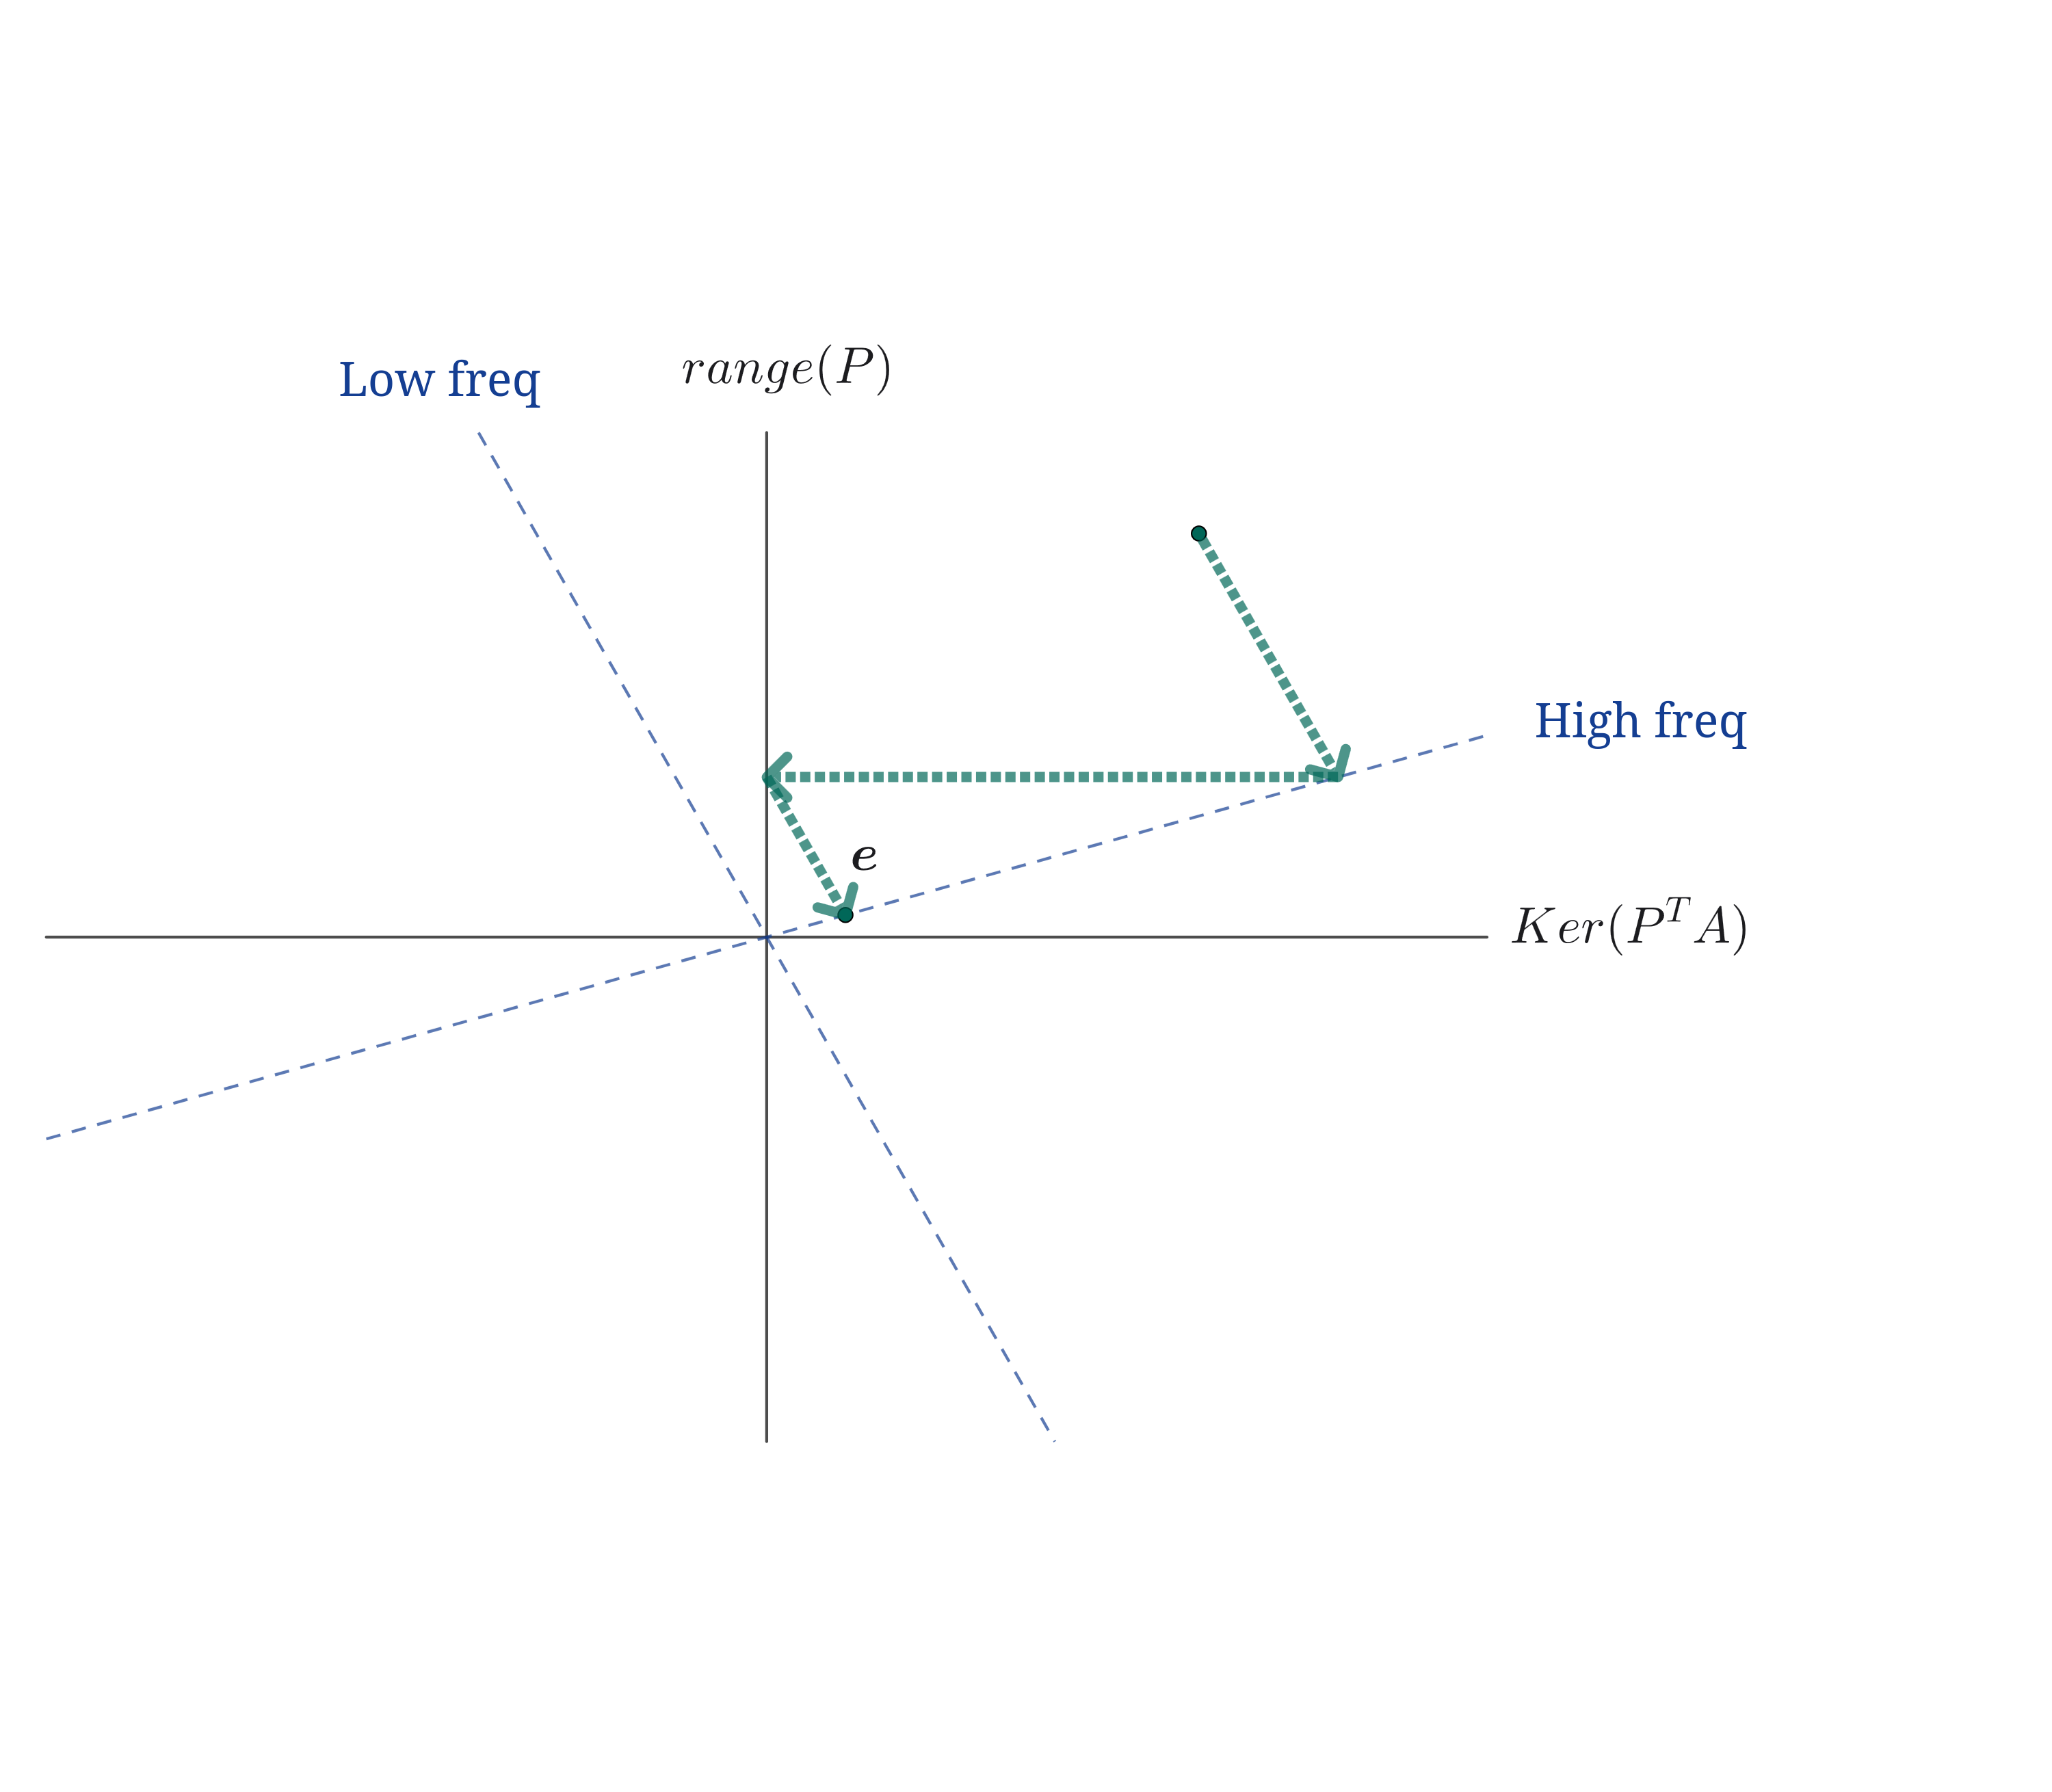
\includegraphics{../pictures/Convergence.png}

\section{algebraic multigrid}

There is no grid: location are unknown or inexistant.

\subsection{algebraic smooth error}

we choose a relaxation method. An error is algebraically smooth when it is not reduced by the smoother.

\begin{align*}
      & Se \approx  e \\ 
 \iff & \left(I - M^{-1}N\right)e \approx  0 \\ 
 \iff & \left(M - N\right)e \approx  0 \\ 
 \iff & Ae = r \approx  0 \\ 
\end{align*}

more rigorously if the smoother satisfies the smoothing property, \\ 
we have $\|r\|_{D^{-1}} \ll  \|e\|_{A}$

% the D norm is there so that the results do not depend on what's in the diagonal of A, the "scale" of the problem
% in the Laplacian case, D is cst*I so it's just the euclidien norm

\begin{align*}
    \|e\|_{A}^{2} & = \langle Ae, e \rangle \\
                  & =  \langle D^{-\frac{1}{2}}Ae, D^{\frac{1}{2}}e \rangle \\
                  & \le \| D^{-\frac{1}{2}}Ae \|_{2} \| D^{\frac{1}{2}}e \| \\
                  & \le \| r \|_{D^{-1}} \| e \|_{D}
\end{align*}

meaning we have $ \|e\|_{A} \ll \|e\|_{D}$ or $\langle Ae,e \rangle \ll \langle De, e \rangle  $

for some smooth error $s = D^{\frac{1}{2}}e$

we have $ \langle Ae,e \rangle = s^{\top}D^{-\frac{1}{2}}AD^{-\frac{1}{2}}s $ and $\langle De, e \rangle = s^{\top}s $

meaning
\begin{align*}
      & s^{\top}\hat{A} s \ll  s^{\top}s \\ 
 \iff & \frac{s^{\top}\hat{A} s}{s^{\top}s} \ll 1 \\ 
 \iff & r_{\hat{A}}(s) \ll 1 \\ 
\end{align*}

with $\hat{A} = D^{-\frac{1}{2}}AD^{-\frac{1}{2}}$

the Rayleigh quotient of a smooth error is small.

This means that smooth errors are a combination of eigenvectors of $\hat{A}$ with small eigenvalues.

% but it is \hat{A} and not A and s and not e ?
% TODO look at: generalized eigenvalue problem

\textbf{Connection with the smoother}

\[
s^{(k+1)} = D^{1/2}\left(I - M^{-1}A\right)D^{-1/2}s^{(k)} = \left(I - \hat{M}^{-1}\hat{A}\right)s^{(k)} = \hat{S}s^{(k)}
\]

Damped Jacobi: $M = \frac{1}{\omega}D$
In this case, $\hat{M} = \frac{1}{\omega}I$

The smoother operator simplifies to: $\hat{S} = I - \omega \hat{A}$

The eigenvalues are $\lambda_i(\hat{S}) = 1 - \omega \lambda_i(\hat{A})$.

For large eigenvalues of $\hat{A}$, $|\lambda_i(\hat{S})| \ll 1$: the smoother is effective

For small eigenvalues, we get $\lambda_i(\hat{S}) \approx 1$: these components form the smooth error, unaffected by the iteration

\subsubsection*{Spectral insight}

we want to compare $\|r\|_{D^{-1}} $ and $\|e\|_{A} = \langle Ae,e \rangle$ when $e$ is a smooth error.

\[
\|r\|_{D^{-1}} = \|Ae\|_{D^{-1}} = \|D^{-\frac{1}{2}}Ae\|_{2} = \|\hat{A}s\|_{2} = \sum_{k}{\lambda_{k}^2c_{k}^{2}}
\]
using the decomposition in an eigenvector basis of $\hat{A}$

interpretation: \\
when the components along high energy modes ($\lambda_{k}$ is big) are important, the norm is huge. \\
when the error is algebraically smooth, $r \approx 0$ and the norm is tiny. 

additionally
\[
\langle Ae,e \rangle = \langle \hat{A}s,s \rangle = \sum_{k}{\lambda_{k}c_{k}^{2}}
\]


if the smoother is effective, only components of eigenvectors of $\hat{A}$ with small eigenvalues remain, ie:

\[
\|r\|_{D^{-1}}^{2} \approx \sum_{\lambda_{k} \le \epsilon}{\lambda_{k}^{2}c_{k}^{2}} \le \epsilon \sum_{\lambda_{k} \le \epsilon}{\lambda_{k}c_{k}^{2}} \approx \epsilon \langle Ae,e \rangle
\]

which means

\[
\|r\|_{D^{-1}} \le \sqrt{\epsilon}\|e\|_{A}
\]

if the smoother is effective $\sqrt{\epsilon} \ll 1$ and we have $\|r\|_{D^{-1}} \ll  \|e\|_{A}$
% that sqrt is bothering me

\subsection{Convergence analysis}

Convergence of a multigrid method requires two hypothesis:

\textbf{The Smoothing Property}: The smoother $S$ reduces high-frequency errors
\[
    \|S e\|_{A}^2 \le \|e\|_{A}^2 - \alpha \|A e\|_{D^{-1}}^2
\]
% see in Hackbusch

\begin{itemize}
    \item This implies $S$ is a contraction in the $A$-norm, and the relaxation would converge
    \item the negative term quantifies the drop: if the error is smooth $A e \approx 0$, and progress stalls \\
    if the error is oscillatory, $\|r\|_{D^{-1}} = \|\hat{A}s\|_{2} = \sum_{k}{\lambda_{k}^2c_{k}^{2}}$ is huge and progress is fast
\end{itemize}

\textbf{The Approximation Property}: The coarse grid can approximate smooth errors

\[
\min_{u_c} \|e - P u_c\|_D^2 \le \beta \|e\|_{A}^2
\]
% the distance between the error and range(P)

\begin{itemize}
    \item if the error is oscillatory, $\|e\|_{A}$ is huge, and the inequality is easily satisfied, regardless of the quality of the interpolation
    \item if $e$ is a smooth error, the interpolation needs to accurately represent it: smooth errors must be near $\range(P)$
\end{itemize}

% the role of the smoother is to take care of the high energy components.
% the two grid operator has to deal with the rest, and for that the low energy modes have to be in range(P)
% in practice this is not "verified", but enforced: range(P) explicitly targets the low energy modes

\textbf{Convergence theorem}

if $\alpha \le \beta$ the iteration converges, with $\| STG \|_A \le \sqrt{1 - \frac{\alpha}{\beta}}$

\textbf{proof}:

by the smoothing property,
\[
    \|S TGe\|_{A}^2 \le \|TGe\|_{A}^2 - \alpha \|A TGe\|_{D^{-1}}^2
\]
using $ V = \range{(P)} \oplus_{A} \nul(P^{T}A) $

for $s = TGe $ in $\range(TG)$, we have $\langle As,Ps\rangle = 0$
\begin{align*}
    \|s\|_A^2 & = \langle As,s - Ps\rangle \\
              & = \langle D^{-\frac{1}{2}}As,D^{\frac{1}{2}}(s - Ps)\rangle \\
    \|s\|_A^2 & \le \|As\|_{D^{-1}}\|s - Ps\|_D \qquad & \text{Cauchy-Schwartz} \\
    \|s\|_A^2 & \le \|As\|_{D^{-1}}\beta\|s\|_A & \text{Approximation Property} \\
    \|TGe\|_A & \le \beta \|ATGe\|_{D^{-1}} & s \in \range(TG), \quad e \in \Omega
\end{align*}

\begin{align*}
    \|S TGe\|_{A}^2 & \le \|TGe\|_{A}^2 - \alpha \|A TGe\|_{D^{-1}}^2 \\
                    & \le \|TGe\|_{A}^2 - \frac{\alpha}{\beta}\|TGe\|_{A}^2 \\ 
                    & \le (1 - \frac{\alpha}{\beta})\|TGe\|_{A}^2 \\
    \|S TGe\|_{A}^2 & \le (1 - \frac{\alpha}{\beta})\|e\|_{A}^2 \qquad & \|TG\| \le 1
\end{align*}

% is TG the projection or there is the pre-smoothing too ?
% does not change the proof\

% what about the edge case where the highest energy modes do not need to be suppressed, because they are handled by the subspace correction
% is it because they are in range(P) ? why ?
% it does not really make sense

\subsection{classic AMG}

\subsubsection*{rational}
\[
    r \approx 0 \implies a_{ii}e_i \approx - \sum_{j \neq i}{a_{ij}e_j}
\]

$e_{i}$ is approximated by a weighted average of its neighbors. \\ 
We focus on the biggest contribution, ie the highest $|a_{ij}|$

strong dependence:
\[
|a_{ij}| \ge \theta \max_{i \ne k}{|a_{ik}|}
\]

if j strongly influence i, it's a good candidate for the interpolation.

\begin{align*}
    \|e\|_A = \sum_{ij}{a_{ij}e_i e_j} & = \frac{1}{2} \sum_{ij}{-a_{ij}\left[{(e_i - e_j)}^2 - e_i^2 - e_j^2\right]} \\ 
                                       & = \frac{1}{2} \sum_{ij}{-a_{ij}{\left(e_i - e_j\right)}^2} + \sum_{i}{\left(\sum_{i}{a_{ij}}\right)e_i^2 }
\end{align*}

for M matrices, the $a_{ij}$ are negative and $ \sum_{i}{a_{ij}} = 0$

and for smooth error $\|e\|_{A} = \epsilon \|e\|_{D} = \epsilon \sum_{i}{a_{ii}e_i^2}$

\[
    \sum_{i}{a_{ii}e_i^2}\left[ \sum_{j \neq i}{\frac{|a_{ij}|}{a_{ii}} \left(\frac{e_i - e_j}{e_i}\right)}^2 - 2\epsilon \right] = 0
\]

meaning most of the time $ \frac{|a_{ij}|}{a_{ii}} {\left(\frac{e_i - e_j}{e_i}\right)}^2 $ is small \\
when i and j are strongly connected $ \frac{|a_{ij}|}{a_{ii}} $ is large so $e_i \approx e_j $

just like in the geometric case, when the error is smooth, local (= strong influence) variation are small.

\subsubsection*{interpolation}

The interpolation is given by:

\begin{equation*}
    {(P \mathbf{e})}i = 
    \begin{cases}
        \hfill e_i & \text{if } i \in C, \\[8pt]
        \displaystyle \sum_{j \in C_i} \omega_{ij} e_j & \text{if } i \in F
    \end{cases}
\end{equation*}

Coarse grid values are directly used. \\
The other are inferred from their strong connexion with the coarse grid.

Once the interpolation is build, the restriction and coarse operator are defined as:

\begin{align*}
      & R = P^{\top} \\ 
      & A_{c} = P^{\top}AP
\end{align*}

This way the correction is optimal in the A-norm:

\begin{align*}
      \|TGe\|_{A} = \|e - \Pi_{A}e\|_{A} & = \min_{w \in \range(P)}{\|e - w\|_{A}} \\ 
                    \|e - Pe_{c}\|_{A}   & = \min_{x \in \Omega_{c}}{\|e - Px\|_{A}}
\end{align*}


by property of the $A$-orthogonal projection on $\range(P)$ $\Pi_{A}$

\section{Non-linear multigrid}

we want to solve
\[
F(u) = 0
\]

\subsection{Newton's multigrid}

from the guess v, we have:
\[
F(v + dv) = F(v) + dF_{v}dv + O(\|dv\|^{2})
\]

if $v + dv$ is the solution, ad we neglect the high order terms:
\[
dv = -dF_{v}^{-1}F(v)
\]

You can solve the linear problem for $dF_{v}dv = -F(v)$ using classic multigrid

\subsection{Full approximation scheme}

The residual equation is more difficult:
\[
A(v + e) - A(v) = r
\]

when projected on the coarse space:
\[
A(P^{\top}v + e_{c}) - A(P^{\top}v) = P^{\top}r
\]

you recursively solve the non-linear problem

\[
A(u_{c}) = A(P^{\top}v) + P^{\top}r
\]

\end{document}
 
% diagnosis: how does the restriction acts on high/low freq nodes ?